\chapter{Optionen der Klasse hbrs-thesis}
\label{chap:klassenoptionen}
Für die Modularität der Klasse wurden einige Optionen eingebaut. Mithilfe dieser Optionen lässt sich das Dokument zum Teil in Optik und Verwendungszweck anpassen. Im Folgenden werden die Optionen mit Beispielen erläutert.

\section{Spracheinstellungen}
Eine Pflichtoption, welche für eine korrekte Worttrennung verwendet werden muss ist die Einstellung der Sprache. Die Sprache kann aktuell nur zwischen englisch und deutsch unterschieden werden. Weitere Anpassungsmöglichkeiten für komplexere bilinguale Dokumente oder andere Spracheinstellungen müssen über die Datei \texttt{hbrs-thesis.cls} manuell eingestellt werden. Angenommen es wird ein Dokument auf Deutsch geschrieben, so muss in Kombination mit dieser Klasse die Option auf \texttt{german} gesetzt werden. Intern werden dann Optionen für die Deutsche Sprache gesetzt. Wird das Dokument auf Englisch geschrieben, so muss \texttt{english} angegeben werden. 

\begin{code}{latex}
\documentclass[german]{hbrs-thesis}
…
\end{code}

Werden bilinguale Spracheinstellungen im Dokument benötigt, müssen in der Klassendatei \texttt{hbrs-thesis.cls} Einstellungen für das Paket \texttt{babel} getroffen werden. Das Paket befindet sich unter der Region \texttt{Required packages}. Ist die Hauptsprache des Dokuments Englisch, kommen aber durchaus Deutsche Begriffe darin vor, eignet sich die Konfiguration \mintinline{latex}{\RequirePackage[ngerman,english]{babel}}. Die zuletzt angegebene Sprache ist die Hauptsprache.

\begin{information}
    Wird die Sprache über die Optionsmöglichkeiten für das Paket \texttt{babel} direkt in \texttt{hbrs-template.cls} geändert, dürfen keine Sprachangaben als Klassenoptionen gesetzt werden.
\end{information}

\section{Stiloptionen}
Die Klasse besitzt ein paar Optionen, um verschiedene Stile anzubieten. Mithilfe der Option \texttt{classicstyle} bzw. \texttt{modernstyle} kann zwischen einer Schriftart mit Serifen und einer serifenlosen Schriftart (was sind Serifen: \url{https://de.wikipedia.org/wiki/Serife}) unterschieden werden. Serifen sollen dem Lesenden helfen die Zeilen besser zu verfolgen, um während des Lesens nicht in der Zeile zu verrutschen, sind aber auf Bildschirmen teilweise schlechter darzustellen. Der Standard ist hier \texttt{modernstyle} und muss somit nicht explizit angegeben.
\begin{showcase}
\begin{code}{latex}
\documentclass[german,classicstyle]{hbrs-thesis}
…
\end{code}
\tcblower
\begin{figure}[H]
    \centering
    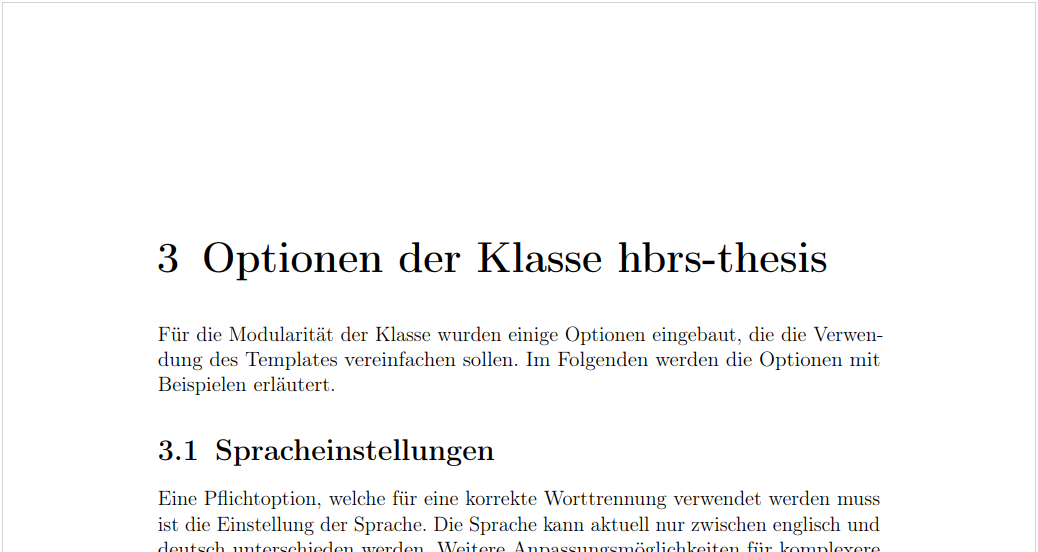
\includegraphics[width=0.8\columnwidth]{assets/images/klassenoptionen/classicstyle.png}
    \caption{Beispielbild für die Option \texttt{classicstyle}.}
\end{figure}
\end{showcase}

Neben dem Stil der Schriftart kann auch zwischen \texttt{report} und \texttt{article} unterschieden werden. Report bietet einzelne Kapitel beschrieben durch \mintinline{latex}{\chapter{…}} welche immer auf einer neuen Seite anfangen. Im Gegensatz dazu bietet \texttt{article} lediglich Abschnitte beschrieben durch \mintinline{latex}{\section{…}}, die nicht jedes Mal auf einer neuen Seite beginnen. Diese beiden Stile können durch die Größe des entstehenden Dokumentes unterschieden werden. Zum Beispiel wird so bei einem Praxisprojektbericht \texttt{article} verwendet wohingegen für eine Thesis \texttt{report} geeignet erscheint. Da die Dokumente nicht doppelseitig ausgedruckt werden entfällt die Option für ein Buchlayout. Diese wird vielleicht später noch hinzugefügt. \textbf{Die Option \texttt{article} ist standardmäßig konfiguriert.} Für eine Thesis sollten die Optionen für die Klasse \texttt{hbrs-thesis} also z.\,B. wie folgt verwendet werden:

\begin{code}{latex}
\documentclass[german,classicstyle,report]{hbrs-thesis}
…
\end{code}

Für den Fall, dass der zweispaltige Stil wie in IEEE- oder ACM-Dokumenten optisch bevorzugt wird, existiert die Option \texttt{twocolumn}. Diese Eignet sich am besten in Kombination der Optionen \texttt{classicstyle} und \texttt{article}. Die entsprechende Konfiguration sieht dann beispielsweise folgendermaßen aus, wobei \texttt{article} Standard ist, also nicht angegeben werden muss:


\begin{showcase}
    \begin{code}{latex}
    \documentclass[german,classicstyle,article,twocolumn]{hbrs-thesis}
    …
    \end{code}
    \tcblower
    \begin{figure}[H]
        \centering
        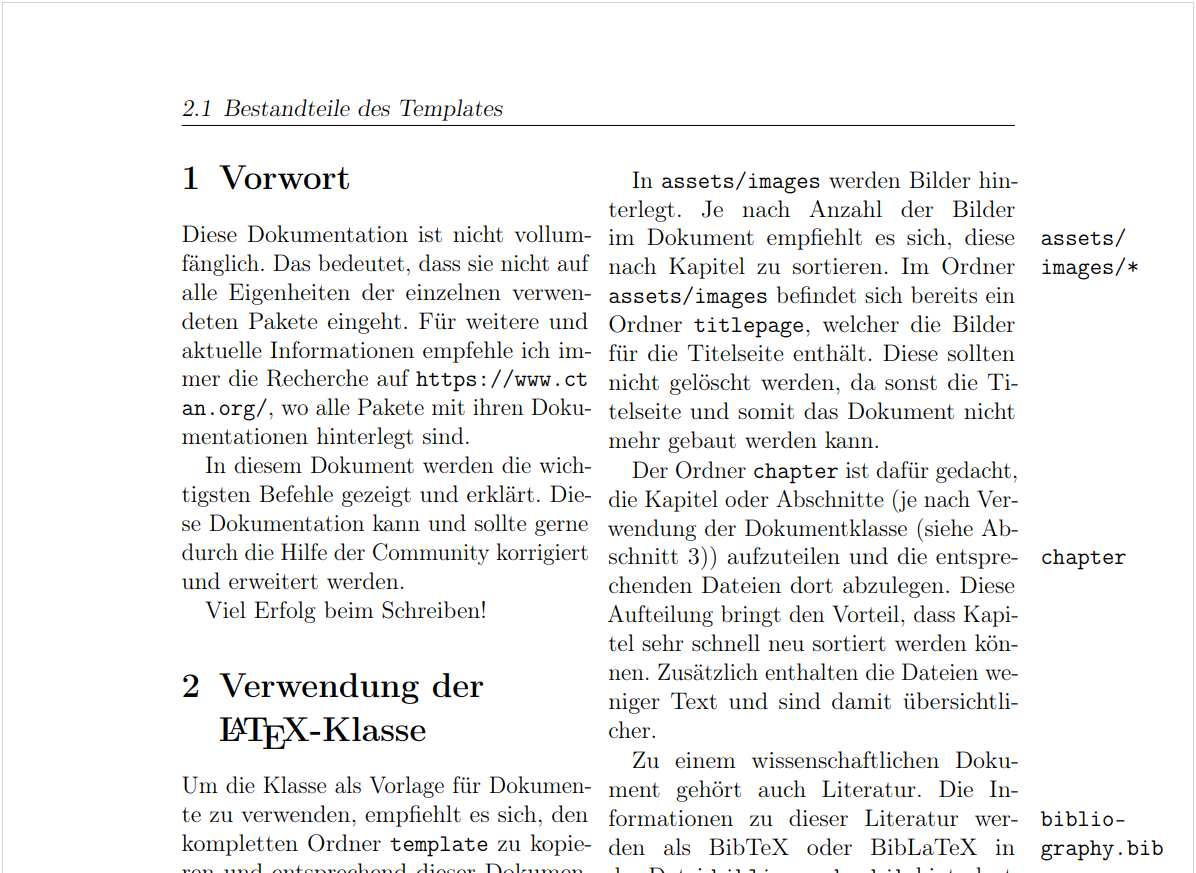
\includegraphics[width=0.8\columnwidth]{assets/images/klassenoptionen/twocolumn_classicstyle_article.png}
        \caption{Beispielbild für die Option \texttt{twocolumn} in Kombination mit \texttt{article} und \texttt{classicstyle}.}
    \end{figure}
\end{showcase}

\section{Glossar und Akronymverzeichnis}
Werden kein Glossar und/oder Akronymverzeichnis verwendet empfiehlt es sich die Option \texttt{noglossaries} in der Klasse zu verwenden. Damit wird das entsprechende Paket nicht geladen, es wird keine Warnung diesbezüglich ausgegeben und das Kompilieren geht eventuell schneller.

\begin{code}{latex}
\documentclass[german,noglossaries]{hbrs-thesis}
…
\end{code}